\documentclass[usenames,dvipsnames]{beamer}
\usetheme{ensam}
\usepackage{pgfplots}
\usepackage{subcaption}
\usepackage{acronym}
\usepackage{tikz}
\usetikzlibrary{calc}
\usepackage{amsmath}
\usepackage {algorithmic}
\usepackage{algorithm}
\usepackage{eqparbox}
\usepackage{mynotations}
\usepackage[font=scriptsize]{caption}
\usetikzlibrary{bayesnet,positioning,calc}
\tikzstyle{obs} = [latent,fill=lightBlue]
\tikzstyle{default}=[draw=sexyRed,thick,rounded corners,text width=0.5in,font=\scriptsize,align=center]
\usepgfplotslibrary{colorbrewer}
\definecolor{ForestGreen}{RGB}{34,139,34}
\newcommand{\comment}[1]{\textcolor{ForestGreen}{#1}}
%algorithmic comment
\renewcommand\algorithmiccomment[1]{%
  \hfill\comment{\#\scriptsize\eqparbox{COMMENT}{#1}}%
}
\renewcommand{\algorithmicrequire}{\textbf{Input:}}
\renewcommand{\algorithmicensure}{\textbf{Output:}}
\title{Relation d'équivalence}
\author{\underline{A.Belcaid}}
\institute{Euromed Fès} 

%tikz bayesian theme
\usetikzlibrary{bayesnet,positioning,calc}
\tikzstyle{obs} = [latent,fill=lightBlue]
\tikzstyle{default}=[draw=sexyRed,thick,rounded corners,text width=0.5in,font=\scriptsize,align=center]
\DeclareMathOperator{\argmin}{argmin}

\pgfplotsset{every tick label/.append style={font=\tiny}}




\begin{document}
\maketitle
\begin{frame}
\tableofcontents
\end{frame}


% Définition {{{ %

\begin{frame}[<+->]
  \frametitle{Définition}
 \begin{block}{Définition}
   Soient $x\in E$ et $y\in F$.\\

   \begin{itemize}
     \item 
   Une relation \alert{$\mathcal{R}$} est une application
   entre $E\times F\rightarrow \{\text{Vrai}, \text{Faux}\}$ qui associe Vrai si
   $x$ et $y$ sont en relation.\\[4pt]
 \item Si le couple $(x,y)$ vérifie (Vrai) la relation on écrit 
   \begin{equation*}
     x\;\mathcal{R}\;y
   \end{equation*}
 \item Dans le cas où $E = F$, on parle d'une relation \textbf{\alert{binaire}}.
   \end{itemize}
 \end{block} 
 \pause
 \begin{center}
 \begin{tikzpicture}[scale=0.9, >=latex]
   \node [point,label=above left:$a$]  at (0,0) (A){};
   \node [point, label=above left:$b$]  at (0.2,-1) (B){};
   \node [point,label=right:$c$]  at (1.4,-1) (C){};
   \node [point,label=above left:$d$]  at (0,-2) (D){};
   \node [point,label=right:$e$]  at (1.2,-2) (E){};
   \path[thick, draw=Apricot, opacity=0.8,->] (A)--(E);
   \path[thick, draw=Apricot, opacity=0.8,->] (B)--(C);
   \path[thick, draw=Apricot, opacity=0.8,->] (B)--(D);
   \path[thick, draw=Apricot, opacity=0.8,->] (D)--(C);
   \path[thick, draw=Apricot, opacity=0.8,->] (C)--(D);
   \path[draw=Apricot, opacity=0.8,->] (A)edge[loop above](A);
   \path[draw=Apricot, opacity=0.8,->] (C)edge[loop above](C);
 \end{tikzpicture}
 \end{center}

\end{frame}
% }}} Définition %
% Propriétées {{{ %
\begin{frame}[<+->]
  \frametitle{Propriétés}
  \small
 Pour une relation \textbf{binaire} dans $E$, on s'intéresse au propriétés
 suivantes:

   \begin{block}{Réflexivité}
          \begin{equation}
            \forall x \in E\quad x\;\mathcal{R}\;x
          \end{equation} 
           \begin{center}
           \begin{tikzpicture}[scale=1, transform shape]
          \node[point, label=right:$x$] (A)  {}; 
          \path[thick, ->,Apricot,->,>=stealth] (A)edge[loop above](A);
           \end{tikzpicture}
         \end{center}
   \end{block}
\pause
   \begin{block}{Symétrie}
          \begin{equation}
            \forall x, y \in E\quad x\;\mathcal{R}\;y\implies y \mathcal{R} x
          \end{equation} 
           \begin{center}
           \begin{tikzpicture}[scale=1, transform shape]
          \node[point, label=left:$x$] (A)  {}; 
          \node[point, label=right:$y$] (B) at (1,0)  {}; 
          \path[thick, ->,Apricot,->,>=stealth,draw] (A)--(B);
          \path[thick, ->,Apricot,->,>=stealth,draw] (B)--(A);
           \end{tikzpicture}
         \end{center}
   \end{block}
\pause
   \begin{block}{Transitivité}
          \begin{equation}
            \forall x, y, z \in E\quad x\;\mathcal{R}\;y \;\text{et}\; y\mathcal{R}z\implies x \mathcal{R} z
          \end{equation} 
           \begin{center}
           \begin{tikzpicture}[scale=0.4]
          \node[point, label=left:$x$] (A)  {}; 
          \node[point, label=right:$y$] (B) at (2,1)  {}; 
          \node[point, label=right:$z$] (C) at (4,0)  {}; 
          \path[thick, ->,Apricot,->,>=stealth,draw] (A)--(B);
          \path[thick, ->,Apricot,->,>=stealth,draw] (B)--(C);
          \path[thick, ->,sexyRed,->,>=stealth,draw] (A)--(C);
           \end{tikzpicture}
         \end{center}
   \end{block}
\end{frame}


\begin{frame}[<+->]
  \frametitle{Relation d'équivalence}
\begin{block}{Définition}
  Soit $\mathcal{R}$ une relation binaire sur $E$. On dit que $\mathcal{R}$ est
  une \textbf{\alert{relation d'équivalence}} si $\mathcal{R}$ est :

  \begin{itemize}
    \item réflexive.
    \item symétrique.
    \item transitive. 
  \end{itemize}
\end{block}
\pause
\begin{center}
\begin{tikzpicture}[scale=1, transform shape]
  \node[point] at (0,0) (A) {};
  \node[point] at (1,0) (B) {};
  \node[point] at (1,1) (C) {};
  \node[point] at (0,1) (D) {};
  \node[point] at (3,0) (F) {};
  \node[point] at (3,1) (G) {};
  \foreach \x in {A,B,C,D,F,G}
  {
    \path[Apricot, draw, ->, >=latex] (\x)edge[loop above](\x);
  }

    \path[Apricot, draw, ->, >=latex] (A)--(B);
    \path[Apricot, draw, ->, >=latex] (A)--(C);
    \path[Apricot, draw, ->, >=latex] (A)--(D);
    \path[Apricot, draw, ->, >=latex] (B)--(C);
    \path[Apricot, draw, ->, >=latex] (B)--(D);
    \path[Apricot, draw, ->, >=latex] (C)--(D);
    \path[Apricot, draw, ->, >=latex] (F)--(G);
    \path[Apricot, draw, ->, >=latex] (G)--(F);
\end{tikzpicture}
\end{center}
\begin{block}{Exemples}
  \begin{itemize}
    \item Si $E=\Z$ et $a\mathcal{R}b \iff ab\neq 0$
    \item Si $E=\Z^{*}$ et $a\mathcal{R}b \iff ab\neq 0$
  \end{itemize} 
\end{block}
\end{frame}

% Autre Exemples {{{ %
\begin{frame}[<+->]
  \frametitle{Exemples}
 \begin{block}{Exemples}
   \begin{enumerate}
     \item On considère $E$ l'ensemble des droites affines dans le plan et la
       relation $\mathcal{R}$ \emph{\alert{être parallèle}}. Cette relation est
       elle un relation d'équivalence?
       \begin{itemize}
         \scriptsize
       \item \textbf{réflexivité}: Une droite est parallèle à elle même.\\[4pt]
         \item \textbf{symétrie}: Si $D$ est parallèle à $D^{'}$, alors $D^{'}$
           est parallèle à $D$.\\[4pt]
         \item \textbf{transitivité}: Si $D_1$ est parallèle à $D_2$ et $D_2$
           est parallèle à $D_3$, alors $D_1$ est parallèle à $D_3$.
       \end{itemize}
     \item La relation \emph{\alert{Être perpendiculaire}} est elle une relation
       d'équivalence?
     \item Relation $\mathcal{R}$ dans $Z$ tel que:
       \begin{equation*}
         x \mathcal{R} y \implies x \text{ \scriptsize est un multiple de }  y
       \end{equation*}
   \end{enumerate}
 \end{block} 
\end{frame}
% }}} Autre Exemples %
% }}} Propriétées %

% Relation d'ordre {{{ %
\begin{frame}[t]
  \frametitle{Relation d'ordre}
 \begin{block}{Définition}
   Une $\mathcal{R}$ dans $E$ est dite relation \textbf{\alert{d'ordre}} si elle vérifie
   les propriétés suivante:

   \begin{itemize}
     \small
   \item \textbf{Réflexive}: $\forall x \in E\quad x \mathcal{R} x$.\\[8pt]
    \item \textbf{Transitivité}: $ x \mathcal{R} y \quad \text{et}\quad
     y\mathcal{R}z\implies x\mathcal{R}z$.\\[8pt]

   \item \textbf{Antisymétrique}: $\left(x\mathcal{R}y\right) \text{ et } \left( y
   \mathcal{R} x\right) \implies x=y$
 \end{itemize}
 \end{block} 
 \begin{center}
 \begin{tikzpicture}[scale=1, transform shape]
   \foreach \x/\y/\z in {0/0/a, 0/1.5/b, 2/1/c, 3/2/d, 4/1.5/e}
   {
     \node[point,label=left:\z] at (\x,\y) (\z){};
     \path[draw,->,>=latex,Apricot, opacity=0.8] (\z)edge[loop above](\z);
   }
   \path[draw,->,>=latex, Apricot, opacity=0.8] (a)--(c);
   \path[draw,->,>=latex, Apricot, opacity=0.8] (a)--(d);
   \path[draw,->,>=latex, Apricot, opacity=0.8] (b)--(c);
   \path[draw,->,>=latex, Apricot, opacity=0.8] (c)--(e);
   \path[draw,->,>=latex, Apricot, opacity=0.8] (d)--(e);
 \end{tikzpicture}
 \end{center}

 \end{frame}


 \begin{frame}[<+->]
   \frametitle{Exemples}
   \begin{itemize}
\item Vérifier que la relation $A \mathcal{R} B \iff A \subset B$ est une
  relation d'ordre.

  \begin{enumerate}
    \small
  \item \textbf{Réflexivité}: $\forall A\in E\quad A \subset A$.\\[8pt]
  \item \textbf{Transitivité}: $\forall A,B,C\in E\quad A \subset B\;\;\text{et
    }B\subset C \implies A\subset C$.\\[8pt]
  \item \textbf{Antisymétrique}: $\forall A, B \in E\quad A \subset B
    \;\;\text{et } B\subset A \implies A=B$.

  \end{enumerate}
  \vspace*{1cm}
\item Même question pour la relation $x\mathcal{R} y \iff x\leq y$ dans $\Z$.
   \end{itemize} 
 \end{frame}


 \begin{frame}[<+->]
   \frametitle{Ordre Total/Partiel}
  \begin{block}{Définition}
    Une relation d'ordre $\mathcal{R}$ sur un ensemble $E$ est dite d'
    \textbf{\alert{ordre total}}. Si deux éléments quelconque de $E$ sont
    \textbf{comparables}.
    \begin{equation}
      \forall x, y \in E\quad (x\mathcal{R} y) ou \left( y \mathcal{R} x\right)
    \end{equation}
    En cas contraire, la relation est dite d'\structure{\textbf{ordre partiel}}
  \end{block} 

  \begin{block}{Exemples}
    \begin{itemize}
      \small
      \item La relation $$x\mathcal{R}y \iff x\leq y$$ est une relation d'ordre
          total dans $\R$.
      \item Par contre la relation $$x\mathcal{R}y \iff x\text{ divise } y$$ est
          une relation d'ordre partiel.
    \end{itemize} 
  \end{block}
 \end{frame}
% }}} Relation d'ordre %
% Classes d'équivalences {{{ %

% Définition classe d'équivalence {{{ %
\begin{frame}[<+->]
  \frametitle{Classe d'équivalence}
 \begin{block}{Définition}
   Pour une relation d'\textbf{équivalence} $\mathcal{R}$ sur un ensemble $E$,
   il est très utile de définir \textbf{\alert{classe d'équivalence}} d'un
   élément $x$ qui contient tous les éléments qui sont en relation avec $x$.

   \begin{equation}
     \cl(x) = \big\{ y\in E \;|\; x \mathcal{R} y\big\}     
   \end{equation}
 \end{block} 

\begin{center}
\begin{tikzpicture}[scale=1, transform shape]
  \node[point] at (0,0) (A) {};
  \node[point] at (1,0) (B) {};
  \node[point] at (1,1) (C) {};
  \node[point] at (0,1) (D) {};
  \node[point] at (3,0) (F) {};
  \node[point] at (3,1) (G) {};
  \foreach \x in {A,B,C,D,F,G}
  {
    \path[Apricot, draw, ->, >=latex] (\x)edge[loop above](\x);
  }

    \path[Apricot, draw, ->, >=latex] (A)--(B);
    \path[Apricot, draw, ->, >=latex] (A)--(C);
    \path[Apricot, draw, ->, >=latex] (A)--(D);
    \path[Apricot, draw, ->, >=latex] (B)--(C);
    \path[Apricot, draw, ->, >=latex] (B)--(D);
    \path[Apricot, draw, ->, >=latex] (C)--(D);
    \path[Apricot, draw, ->, >=latex] (F)--(G);
    \path[Apricot, draw, ->, >=latex] (G)--(F);
    \node[rounded corners, thick, sexyRed, draw, fit=(A)(C), label=left:$\cl(x_1)$]{};
    \node[rounded corners, thick, lightBlue, draw, fit=(G)(F),
      label=right:$\cl(x_2)$]{};
\end{tikzpicture}
\end{center}
\begin{itemize}
  \item On trouve aussi la notation $\overline{x}  =\cl\left(x\right)\subset E$.
\end{itemize}
\end{frame}


\begin{frame}[<+->]
  \frametitle{Propriétés}
 \begin{block}{Propriétés}
   \begin{itemize}
     \item $\cl(x) = \cl(y) \iff x \mathcal{R} y$.\\[8pt]
       \item $\forall x,y \in E \quad  \big(\cl(x) =\cl(y)\big) \text{ ou }
         \big(\cl(x)\cap
         \cl(y)=\emptyset\big)$.
   \end{itemize} 
 \end{block} 
 \begin{block}{Partition}
   
   Soit un ensemble $E$ et un ensemble $\{E_i\}$ des parties de $E$. On dit que
   $\{E_i\}$ forment une \textbf{\alert{partition}}  de $E$ si:
   \begin{equation*}
     \left\{ \begin{array}{ll}
         \cup_i E_i = E & \\
         E_i \cap E_j=\emptyset & (i \neq j)\\
     \end{array}\right.
   \end{equation*}
 \end{block}
 \begin{center}
 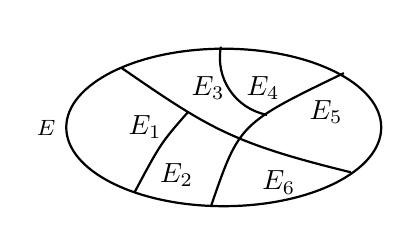
\begin{tikzpicture}[scale=1, transform shape]
   \node[ellipse, minimum width=4cm, minimum height=2cm, draw, thick,
     label=left:$E$]   {};
   \node[] (A) at (-1.42,0.84){};
   \node[] (B) at (-1.2,-0.95){};
   \node[] (C) at (0,1.15){};
   \node[] (D) at (-0.2,-1.11){};
   \node[] (E) at (1.65,0.75){};
   \node[] (F) at (1.74,-0.6){};
   \draw[thick](A)..controls (-0.2,0) and (0.1,-0.2) ..(F);
   \draw[thick](B)..controls (-0.8,-0.2)..(-0.45,0.2);
   \draw[thick] (D)..controls (0.2,0.05)..(E);
   \draw[thick] (C)edge[bend right=45](0.55,0.16);
   \node at (-1,0) {$E_1$};
   \node at (-0.6,-0.6) {$E_2$};
   \node at (-0.2,0.5) {$E_3$};
   \node at (0.5,0.5) {$E_4$};
   \node at (1.3,0.2) {$E_5$};
   \node at (0.7,-0.7) {$E_6$};
 \end{tikzpicture}
 \end{center}
\end{frame}

\begin{frame}[<+->]
  \frametitle{Exemple partition}
 \begin{block}{Exemple 1}
   \small
   On considère la relation $\mathcal{R}$ des ensembles des étudiants qui relie
   deux étudiants s'ils ont le \emph{même age}.\\[4pt]

   \begin{itemize}
     \scriptsize
     \item Deux étudiants appartient à la même classe s'ils ont le même
       age.\\[4pt]
     \item Deux étudiants sont soit dans la même classe soit à deux classes
       \alert{\textbf{différentes}}.\\[4pt]
     \item La classe peut être décomposé en différentes parties selon leur age.
   \end{itemize}
 \end{block} 
 \pause
 \vspace*{1cm}
 \begin{columns}
   \begin{column}{0.5\textwidth}
     \centering
     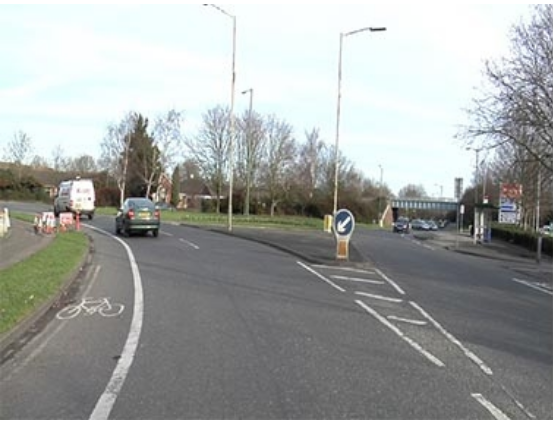
\includegraphics[width=4cm, height=3cm]{./segmentation_01.jpg}
   \end{column}
   \begin{column}{0.5\textwidth}
     \centering
     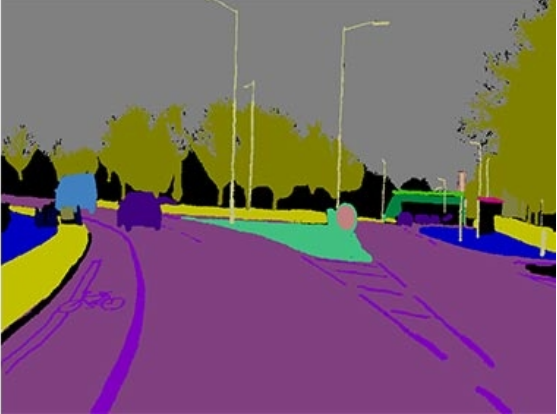
\includegraphics[width=4cm, height=3cm]{./segmentation_02.jpg}
   \end{column}
 \end{columns}
\end{frame}
 
% }}} Définition classe d'équivalence %
% }}} Classes d'équivalences %
% Ensemble Z / nZ {{{ %
\begin{frame}[<+->]
  \frametitle{Ensemble $\Z/n\Z$}
  
  \begin{block}{Définition}
    Soit $ E = \Z$, nous définissons la relation suivante:

    \begin{equation}
      a \equiv b (\text{mod } n) \iff  \big(a - b\big) \text{ \scriptsize est un multiple de } n
    \end{equation}
  \end{block}
  \begin{itemize}
    \small
  \item \textbf{Exemple}: $1\equiv 5 (\text{mod } 2)$ et $3\equiv 10 (\text{mode
    } 3)$.
    \item Vérifier que $\equiv$ est une relation d'
      \textbf{\alert{équivalence}}.
    \item La \textbf{classe d'équivalence} d'un nombre note $\overline{a}$ est
      donné par:
      \begin{eqnarray*}
        \overline{a} &=&\big\{ b\in \Z\;|\; b \equiv a (\text{mode } n)\big\} \\
        \overline{a} &=& \big\{ a + kn \;|\; k\in \Z\big\}  = a + k\Z
      \end{eqnarray*}
    \item Une \textbf{partition} par cette relation  de $\Z$ qu'on note
      \alert{$\mathbf{\Z/n\Z}$}  est donnée par:
      \begin{equation*}
        \Z/n\Z = \big\{ \overline{0}, \overline{1},\ldots, \overline{n-1}\big\} 
      \end{equation*}
  \end{itemize}
\end{frame}
\begin{frame}[t]
  \frametitle{Exercices rapides}

  \begin{block}{Exercices}
    \begin{itemize}
      \item Lister les éléments de l'ensemble $\Z/7\Z$
    \end{itemize}
  \end{block}
  
\end{frame}
% }}} Ensemble Z / nZ %
\end{document}
